% --------------------------------------------------
%  TALLER DE INTRODUCCIÓN A LaTeX
%  https://github.com/mianfg/latex-intro
%
%  Sesión 1 -> Presentación
%
%  Autor: Miguel Ángel Fernández Gutiérrez, @mianfg
%  Fecha: 20 febrero, 2019
% --------------------------------------------------

% Tipo de documento (presentación)
\documentclass[10pt, xcolor=table]{beamer}

% Cargar el tema
\usetheme{metropolis}

%  __________
% |          |
% | Paquetes |
% |__________|

% Paquetes de idioma
\usepackage[utf8]{inputenc}
\usepackage[spanish, es-tabla, es-lcroman, es-noquoting]{babel}

% Paquete para código fuente
% LISTINGS
\usepackage{listings}
\usepackage{lipsum}
\usepackage{courier}

% Colores para los bloques de código
\definecolor{codegreen}{rgb}{0,0.6,0}
\definecolor{codegray}{rgb}{0.5,0.5,0.5}
\definecolor{codepurple}{rgb}{0.58,0,0.82}
\definecolor{backcolour}{rgb}{0.95,0.95,0.92}
\lstdefinestyle{mystyle}{
	backgroundcolor=\color{backcolour},   
	commentstyle=\color{codegreen},
	keywordstyle=\color{blue},
	numberstyle=\tiny\color{codegray},
	stringstyle=\color{codepurple},
	basicstyle=\footnotesize\ttfamily,
	breakatwhitespace=false,         
	breaklines=true,                 
	captionpos=b,                    
	keepspaces=true,                 
	numbers=left,                    
	numbersep=5pt,                  
	showspaces=false,                
	showstringspaces=false,
	showtabs=false,                  
	tabsize=4
}
\lstset{style=mystyle}

% Paquete de numeración en Beamer
\usepackage{appendixnumberbeamer}

% Paquete de uso para plantilla
\usepackage{booktabs}
\usepackage[scale=2]{ccicons}

% Paquete para controlar espacios
\usepackage{xspace}
\newcommand{\themename}{\textbf{\textsc{metropolis}}\xspace}

% Paquetes para matemáticas
\usepackage{amsmath}    % Paquete básico de matemáticas
\usepackage{amsthm}     % Teoremas
\usepackage{mathrsfs}   % Fuente para ciertas letras utilizadas en matemáticas

% Paquetes para fuentes
\usepackage{newpxtext, newpxmath}   % Fuente similar a Palatino
\usepackage{FiraSans}               % Fuente sans serif
\usepackage[T1]{fontenc}
\usepackage[italic]{mathastext}     % Utiliza la fuente del documento
                                    % en los entornos matemáticos

%  ________________________
% |                        |
% | Configuración del tema |
% |________________________|

% Configuración básica del tema
\metroset{
  % tema oscuro ('dark') o claro ('light'). No tiene efecto al usar la
  % paleta de colores más adelante
  background=light,
  % 'none' para eliminar la diapositiva inicial de cada sección
  sectionpage=progressbar,
  % 'progressbar' o 'simple' para añadir una diapositiva inicial a cada subsección
  subsectionpage=none,
  % contador de página: 'none', 'counter' o 'fraction'
  numbering=none,
  % barra de progreso: 'none', 'head', 'frametitle' o 'foot'
  progressbar=frametitle,
  % fondo de los bloques estilo teorema: 'transparent' o 'fill'
  block=fill,
}

% Paleta de colores
\definecolor{accent}{HTML}{009688}
\colorlet{darkaccent}{accent!70!black}
\definecolor{foreground}{RGB}{0, 0, 0}
\definecolor{background}{RGB}{255, 255, 255}

% Insertar los colores en el tema
\setbeamercolor{normal text}{fg=foreground, bg=background}
\setbeamercolor{alerted text}{fg=darkaccent, bg=background}
\setbeamercolor{example text}{fg=foreground, bg=background}
\setbeamercolor{frametitle}{fg=background, bg=accent}

\setbeamercolor{headtitle}{fg=background!70!accent,bg=accent!90!foreground}
\setbeamercolor{headnav}{fg=background,bg=accent!90!foreground}
\setbeamercolor{section in head/foot}{fg=background,bg=accent}

\defbeamertemplate*{headline}{miniframes theme no subsection}{
  % Caja para mostrar título y autor encima de cada diapositiva
  % Nosotros no 
  %% \begin{beamercolorbox}[ht=2.5ex,dp=1.125ex,
  %%     leftskip=.3cm,rightskip=.3cm plus1fil]{headtitle}
  %%   {\usebeamerfont{title in head/foot}\insertshorttitle}
  %%   \hfill
  %%   \leavevmode{\usebeamerfont{author in head/foot}\insertshortauthor}
  %% \end{beamercolorbox}
  %% \begin{beamercolorbox}[colsep=1.5pt]{upper separation line head}
  %% \end{beamercolorbox}

  % Caja para mostrar navegación encima de cada diapositiva
  \begin{beamercolorbox}{headnav}
    \vskip2pt\insertnavigation{\paperwidth}\vskip2pt
  \end{beamercolorbox}
  \begin{beamercolorbox}[colsep=1.5pt]{lower separation line head}
  \end{beamercolorbox}
}

%  _________
% |         |
% | Ajustes |
% |_________|

% Fijar tabla a posición
\usepackage{array}
\newcolumntype{L}[1]{>{\raggedright\let\newline\\\arraybackslash\hspace{0pt}}m{#1}}
\newcolumntype{C}[1]{>{\centering\let\newline\\\arraybackslash\hspace{0pt}}m{#1}}
\newcolumntype{R}[1]{>{\raggedleft\let\newline\\\arraybackslash\hspace{0pt}}m{#1}}

%  ________
% |        |
% | Título |
% |________|

\title{Programación dinámica}
\subtitle{Algorítmica. \alert{Práctica 4}}
\date{}
\author{Celia Arias Martínez\\Miguel Ángel Fernández Gutiérrez\\Sergio Quijano Rey\\Lucía Salamanca López\\[4pt]\footnotesize{segfault}}
\titlegraphic{\hfill
\includegraphics[width=2.5cm]{ugrlogo-dark.pdf}}

%  ___________
% |           |
% | Documento |
% |___________|

\begin{document}

\maketitle

\begin{frame}{Contenidos}
	\setbeamertemplate{section in toc}[sections numbered]
	\tableofcontents[]
\end{frame}


\section{Introducción}

\begin{frame}{Objetivo}
Apreciar la utilidad de la \emph{programación dinámica para} resolver problemas que involucran recursividad, de forma eficiente.
\begin{itemize}
	\item \textbf{Problema escogido}: Subsecuencia de caracteres más larga\\(\textit{LCS} o \textit{Longest Common Subsequence}).
\end{itemize}

\end{frame}

\section{Problema: LCS (subsecuencia más larga)}
\begin{frame}{Descripción del problema}
\begin{center}
	\textbf{\large{Problema de la subsecuencia más larga (LCS)}}
\end{center}

Dadas dos secuencias de caracteres, encontrar la máxima subsecuencia de caracteres común que aparecen en ambas cadenas de izquierda a derecha (no necesariamente de forma contigua).
\end{frame}

\begin{frame}[fragile]{Descripción del problema}
\vspace{0.55cm}
	\begin{center}
	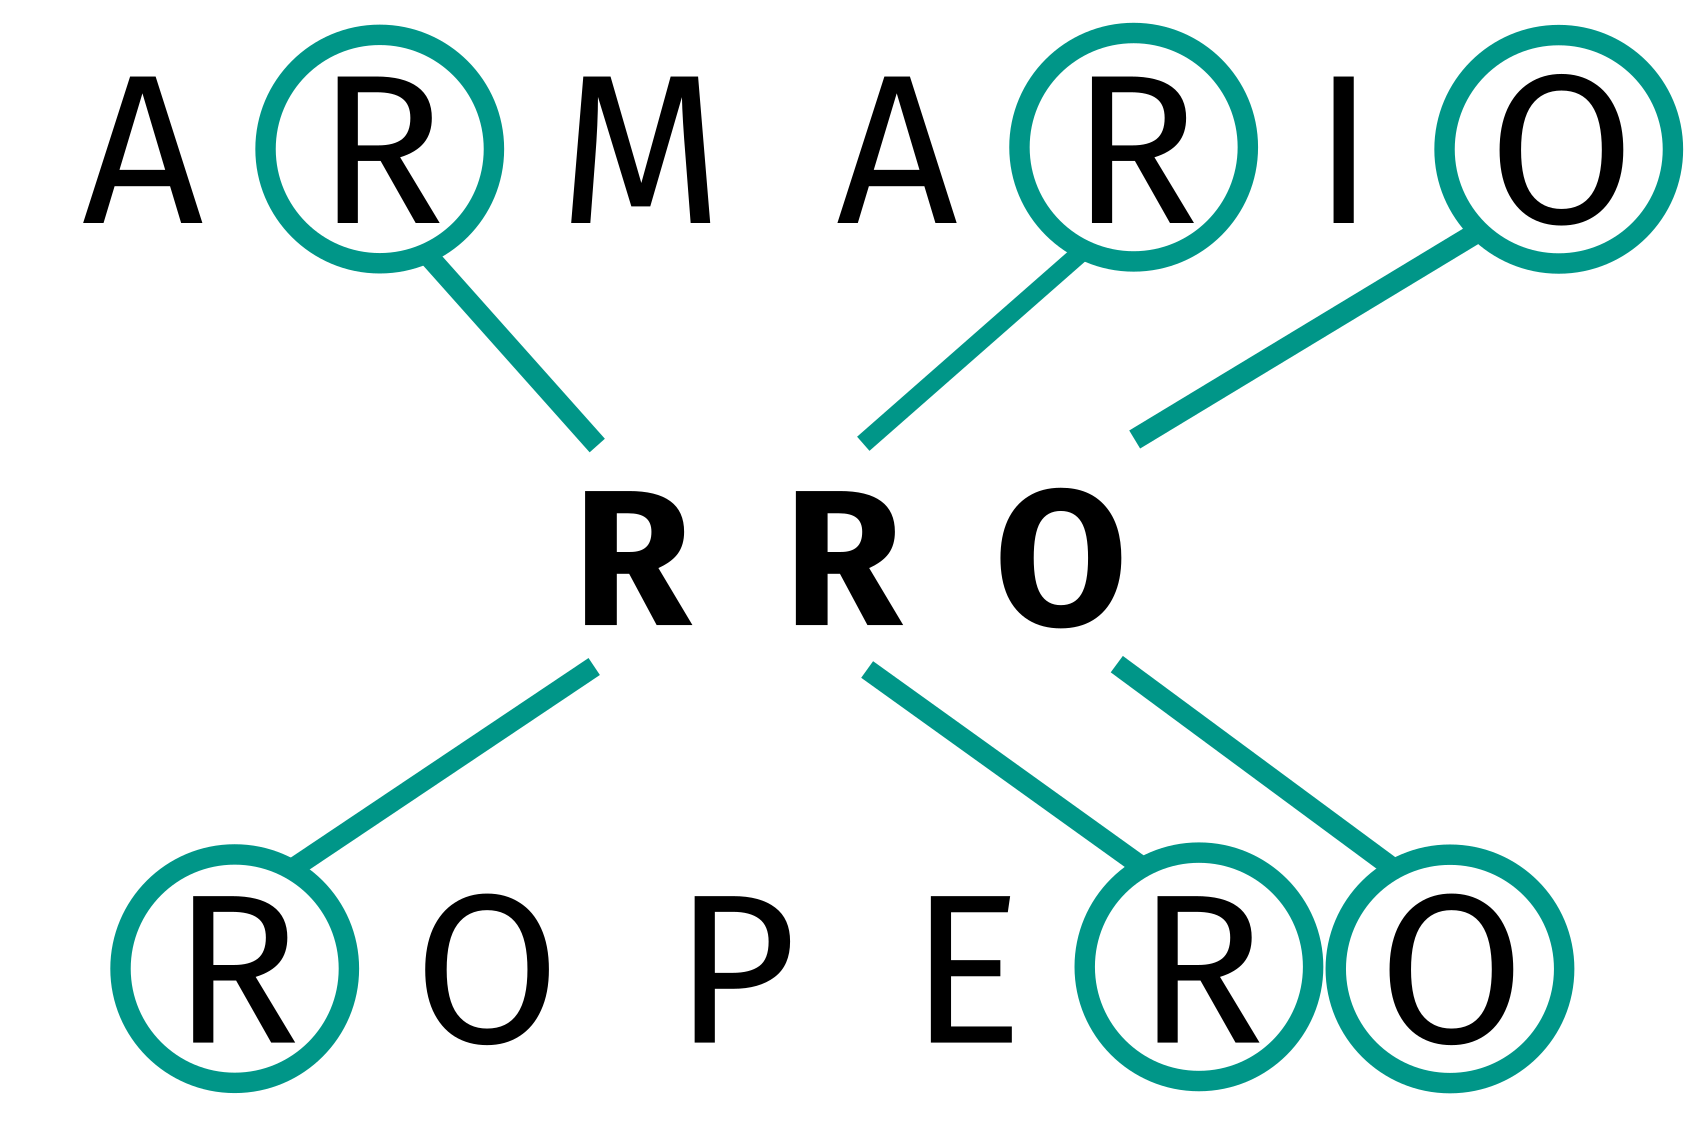
\includegraphics[width=200px]{./resources/diagrama.png}
\end{center}
\end{frame}

\begin{frame}{Diseño de la solución}
Aplicamos programación dinámica en cuatro fases:

\begin{enumerate}
	\item Verificación de la naturaleza $n$-etápica del problema.
	\item Verificación del principio de optimalidad de Bellman.
	\item Planteamiento de una recurrencia. 
	\item Cálculo de la solución.
\end{enumerate}
\end{frame}

\begin{frame}{Diseño de la solución. \normalfont{Naturaleza $n$-etápica del problema}}
El resultado es consecuencia de una sucesión de decisiones: en la etapa \textit{n} debemos elegir qué cadena de caracteres dejamos fija y qué puntero movemos hacia la derecha. 

Una \textbf{solución optimal} es aquella que proporcione la subsecuencia de caracteres más larga.
\end{frame}

\begin{frame}{Diseño de la solución. \normalfont{Principio de optimalidad de Bellman}}
\textbf{Función a maximizar}: número de caracteres en común en las dos subsecuencias. Tendremos, por tanto, en la etapa $n$:
$$
f_n(i,j) = \text{máx}\{f(i-1,j),f(i,j-1)\}+\delta_{ij}$$
\vspace{-0.8cm}
\begin{itemize}
	\item $\delta_{ij}$: función que dados dos índices (de distintas subcadenas), devuelve 1 si coinciden y 0 en otro caso.
\end{itemize}

\textbf{Caso base}:
$$
f_1(i,j) = \text{máx}\{\delta_{ij}\} = \delta_{ij}
$$
Es obvio que la solución proporcionada en la etapa $n$ es optimal, pues estamos calculando el máximo de dos funciones optimales.
\end{frame}

\begin{frame}{Diseño de la solución. \normalfont{Planteamiento de recurrencia}}
\begin{center}
	\textbf{Recurrencia planteada}
\end{center}
$$ LCS{[i,j]}= \left\{\begin{matrix} 1+LCS[i-1,j-1] \\ \text{máx}\{LCS[i-1,j],LCS[i,j-1]\}\end{matrix}\right. $$

Conseguimos asegurar el principio de optimalidad: si estamos en la etapa $n$, las decisiones tomadas hasta la etapa $n-1$ son óptimas.
\end{frame}

\begin{frame}[fragile]{Diseño de la solución. \normalfont{Cálculo de solución}}
\begin{center}
	\textbf{\large{\texttt{constructLCSMat}}}
\end{center}
\begin{lstlisting}[language=C]
vector<vector<int> > constructLCSMat(string str1, string str2) {
	vector<vector<int> > lcs_mat(str1.size() + 1,
		vector<int>(str2.size() + 1, 0));
	
	for ( int i = 1; i <= str1.size(); i++ ) {
		for ( int j = 1; j <= str2.size(); j++ ) {
			if ( str1[i-1] == str2[j-1] )
				lcs_mat[i][j] = 1 + lcs_mat[i-1][j-1];
			else
				lcs_mat[i][j]
					= max(lcs_mat[i-1][j], lcs_mat[i][j-1]);
		}
	}
	
	return lcs_mat;
}
\end{lstlisting}
\end{frame}

\begin{frame}[fragile]{Diseño de la solución. \normalfont{Cálculo de solución}}
\begin{center}
	\textbf{\large{\texttt{constructLCSMat}}}
\end{center}
Creamos la matriz usada para encontrar el número de caracteres y las letras que conforman la máxima subsecuencia en común.

$$
\begin{matrix}
 & \begin{matrix} \textcolor{white}{....}\vspace{0.3cm}&\text{{a}} & \text{{r}} & \text{{m}} & \text{{a}} & \text{{r}} & \text{{i}} & \text{{o}} \end{matrix} \\
\begin{matrix}\\ \text{{r}}\\\text{{o}}\\\text{{p}}\\\text{{e}}\\\text{{r}}\\\text{{o}} \end{matrix} & \left(\begin{matrix}
0 & 0 & 0 &0&0&0&0&0\\
0&0&1&1&1&1&1&1\\
0&0&1&1&1&1&1&2\\
0&0&1&1&1&1&1&2\\
0&0&1&1&1&1&1&2\\
0&0&1&1&1&2&2&2\\
0&0&1&1&1&2&2&3\\
\end{matrix}\right)
\end{matrix}
$$
\end{frame}

\begin{frame}[fragile]{Diseño de la solución. \normalfont{Cálculo de solución}}
\begin{center}
	\textbf{\large{\texttt{getLCS}}}
\end{center}
\begin{lstlisting}[language=C]
string getLCS(string str1, string str2) {
	vector<vector<int> > lcs_mat = constructLCSMat(str1, str2);
	string word;
	
	int i = str1.size(), j = str2.size();
	
	while ( j > 0 ) {
		j--;
		if ( lcs_mat[i][j] != lcs_mat[i][j+1] ) {
			word = str2[j] + word;
			i--;
		}
	}
	
	return word;
}
\end{lstlisting}
\end{frame}

\begin{frame}[fragile]{Diseño de la solución. \normalfont{Cálculo de solución}}
\begin{center}
	\textbf{\large{\texttt{getLCS}}}
\end{center}
Llamamos a la función \texttt{constructLCSMat} para construir la matriz, luego la recorremos para encontrar las letras de la LCS.
$$
\begin{matrix}
 & \begin{matrix} \textcolor{white}{....}\vspace{0.3cm}&\text{{a}} & \text{\textcolor{red}{r}} & \text{{m}} & \text{{a}} & \text{\textcolor{red}{r}} & \text{{i}} & \text{\textcolor{red}{o}} \end{matrix} \\
\begin{matrix}\\ \text{\textcolor{red}{r}}\\\text{{o}}\\\text{{p}}\\\text{{e}}\\\text{\textcolor{red}{r}}\\\text{{\textcolor{red}{o}}} \end{matrix} & \left(\begin{matrix}
0 & 0 & 0 &0&0&0&0&0\\
0&0&\textbf{\textcolor{red}{1}}&1&1&1&1&1\\
0&0&\textbf{1}&1&1&1&1&2\\
0&0&\textbf{1}&1&1&1&1&2\\
0&0&\textbf{1}&\textbf{1}&\textbf{1}&1&1&2\\
0&0&1&1&1&\textbf{\textcolor{red}{2}}&\textbf{2}&2\\
0&0&1&1&1&2&2&\textbf{\textcolor{red}{3}}\\
\end{matrix}\right)
\end{matrix}
$$
\end{frame}

\begin{frame}[fragile]{Diseño de la solución. \normalfont{Cálculo de solución}}
$$
\begin{matrix}
 & \begin{matrix} \textcolor{white}{....}\vspace{0.3cm}&\text{{a}} & \text{\textcolor{red}{r}} & \text{{m}} & \text{{a}} & \text{\textcolor{red}{r}} & \text{{i}} & \text{\textcolor{red}{o}} \end{matrix} \\
\begin{matrix}\\ \text{\textcolor{red}{r}}\\\text{{o}}\\\text{{p}}\\\text{{e}}\\\text{\textcolor{red}{r}}\\\text{{\textcolor{red}{o}}} \end{matrix} & \left(\begin{matrix}
0 & 0 & 0 &0&0&0&0&0\\
0&0&\textbf{\textcolor{red}{1}}&1&1&1&1&1\\
0&0&\textbf{1}&1&1&1&1&2\\
0&0&\textbf{1}&1&1&1&1&2\\
0&0&\textbf{1}&\textbf{1}&\textbf{1}&1&1&2\\
0&0&1&1&1&\textbf{\textcolor{red}{2}}&\textbf{2}&2\\
0&0&1&1&1&2&2&\textbf{\textcolor{red}{3}}\\
\end{matrix}\right)
\end{matrix}
$$

\begin{center}
	\text{\large ``rro''}\\	
	(\textbf{r}ope\textbf{ro}, a\textbf{r}ma\textbf{r}i\textbf{o})
\end{center}
\end{frame}

\begin{frame}[fragile]{Análisis empírico}
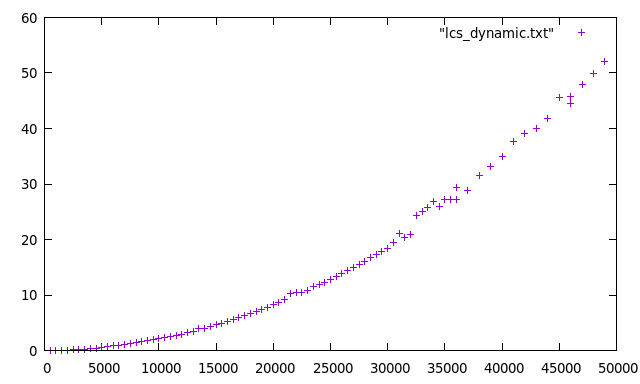
\includegraphics[width=\textwidth]{./../Graficas/lcs_dinamic.png}
\begin{center}
	\footnotesize{Datos empíricos: algoritmo dinámico}
\end{center}
\end{frame}

\begin{frame}[fragile]{Comparación: \normalfont{dinámico vs. fuerza bruta}}
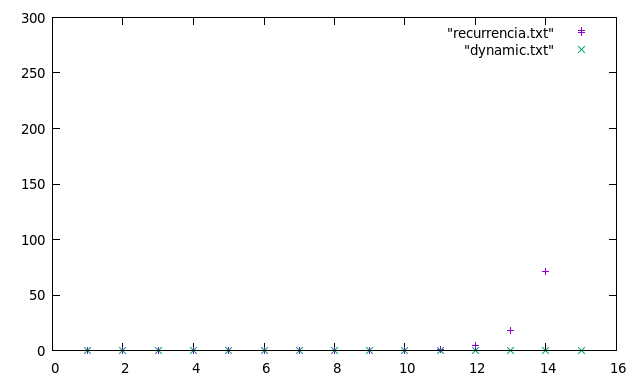
\includegraphics[width=\textwidth]{./../Graficas/comparacion.png}
\begin{center}
	\footnotesize{Comparación: algoritmo dinámico vs fuerza bruta}
\end{center}
\end{frame}


\section{Conclusiones}

\begin{frame}{Conclusiones}
Con esta práctica, hemos aprendido a crear algoritmos de programación dinámica para resolver problemas encadenados que podemos optimizar, comprobando las condiciones que han de verificar.

Al contrario de algoritmos simples de recurrencia en cada iteración no hay que volver a comprobar todas las soluciones posibles, ya que hemos guardado las mejores soluciones anteriores.

Especial relevancia para encontrar solución \textbf{óptima}.
\end{frame}

\end{document}
